\section{Raumerkennung}

Die Raumerkennung ist der wichtigste Aspekt unserer Anwendung.
Die zugrundeliegende Idee ist, dass stationäre Beacons in den
relevanten Räumen platziert werden. Anschließend werden diese
Räume einmalig vermessen, um ein Modell zur Erkennung der
Räume zu erstellen.
Dabei ist zu beachten, dass wir im Gegensatz zu anderen Projekten
im Bereich In-Door-Lokalisation keine Informationen über die
Räume oder die Position der Beacons besitzen. Aus diesem Grund
beschränken wir die Genauigkeit der Positionsbestimmung auf
Raumebene.

Im Folgenden wird beschrieben, wie wir die Messung der Beacons
durchgeführt haben. Auf Basis der ersten Messwerte analysieren
wir, ob diese Informationen ausreichen, um eine Raumzuordnung
zu ermöglichen. Nachdem die Machbarkeit nachgewiesen wurde,
entwickeln wir einen Lösungsansatz für das Problem.
Abschließend stellen wir unsere konkrete Implementierung vor.

\subsection{Messung}

Eine \textbf{Einzelmessung} bezieht sich auf die Signalstärke eines Beacons.
Die Signalstärke wird in der Einheit RSSI (Received Signal Strength Indication)
gemessen. Da diese von der Implementierung des Empfängers abhängig ist,
normalisieren wir die Werte auf das Intervall $[0, 1] \subset \mathbb{R}$, wobei
$0$ kein Signal und $1$ maximale Signalstärke bedeutet.

Unter einer \textbf{Messung} verstehen wir einen Vektor von Einzelmessungen,
welche gleichzeitig aufgenommen wurden.

In der Realität ergeben sich zwei Probleme, bei der Messung nach obigem
Schema:
\begin{enumerate}
	\item Einzelmessungen werden vom Bluetooth-Empfänger der betrachteten
	  Geräte ca. jede Sekunde durchgeführt. Dabei kommen Einzelmessungen nicht
	  gleichzeitig für alle Beacons in Reichweite an, sondern verteilt über
	  den Zeitraum von einer Sekunde. Es stellt sich also die Frage, was
	  gleichzeitig, bei der Definition einer Messung bedeutet.
	\item Es kann vorkommen, dass ein Beacon in Reichweite ist, aber in der
	  letzten Sekunde nicht wahrgenommen wurde. Das würde bedeuten, dass ein
	  einziger Aussetzer den Beacon als nicht erreichbar in der Einzelmessung
	  darstellt.
\end{enumerate}

Um beide Probleme zu lösen, führen wir den Begriff der \textbf{Pseudogleichzeitigkeit} ein.
Einzelmessungen sind pseudogleichzeitig erfolgt, wenn diese nicht länger als 
$t_g$ zurückliegen. Dabei wird $t_g > t_m$ gewählt, um einzelne Aussetzer von Beacons
auszugleichen.

\begin{figure}[tbh]
\centering
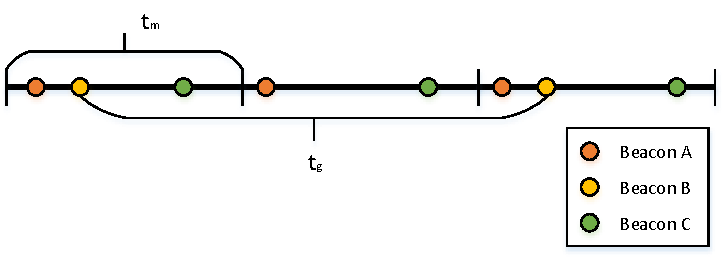
\includegraphics[width=1.0\linewidth]{Bilder/Lok-Messung}
\caption{Pseudogleichzeitigkeit bei Messungen}
\label{fig:Lok-Messung}
\end{figure}

Abbildung \ref{fig:Lok-Messung} zeigt ein Zeitintervall für drei Messungen. Die
Punkte auf dem Zeitstrahl deuten eine Einzelmessung für ein bestimmtes Beacon
an.
Man sieht, dass in der zweiten Messung kein Signal für Beacon B empfangen wurde.
Da jedoch die letzte Messung dieses Beacon weniger als $t_g$ zurückliegt, tragen
wir in der Messung den Wert aus der letzten Messung ein.
In unserem Projekt haben wir $t_g = 2 \cdot t_m$ gewählt, so dass ein nicht mehr
erreichbarer Beacon spätestens nach zwei Messintervallen als nicht vorhanden
erkannt wird.

\subsection{Machbarkeitsanalyse}

Nachdem wir unseren Messvorgang definiert haben, analysieren wir anhand
einer einfachen Raumerkennung mit zwei Räumen und zwei Beacons, ob eine
Unterscheidung der Räume anhand der Messungen möglich ist.
Dazu werden wir die Verteilung der Messwerte sowohl statistisch als
auch grafisch aufbereiten.

In dieser Analyse haben wir zwei Räume gescannt, die im Folgenden als
Küche und Flur bezeichnet wurden. In jedem Raum wurde ein Beacon platziert.
Die Beacons hatten folgende Bluetooth-Adressen:
\begin{itemize}
	\item 7C:2F:80:8D:E2:3B (platziert in Küche)
	\item 7C:2F:80:8D:E2:45 (platziert in Flur)
\end{itemize}
Da sich die Adressen nur in der letzten Stelle unterscheiden, referenzieren
wir diese Beacons im folgenden nur mit diesem Teil der Adresse, d. h.
3B und 45.

\subsubsection{Statistische Aufbereitung}

Als erstes betrachten wir den Minimal-, Maximal, Mittelwert und die Standardabweichung für jeden
Beacon in jedem Raum. Diese bestimmen wir per SQL aus der SQLite-Datenbank der Messwerte.
Da die Messwerte in der Datenbank nicht normalisiert abgelegt wurden, sind die Werte
in Tabelle \ref{tab:sql-analyze} nicht normalisiert.

\begin{table}[h]
	\caption{SQL-Analyse der ersten Messung}
	\label{tab:sql-analyze}
	\begin{tabular}{|c|c|c|c|c|c|}
		\hline \textbf{Raum} & \textbf{Tag} & \textbf{min(RSSI)} & \textbf{max(RSSI)} & \textbf{avg(RSSI)} & \textbf{stddev(RSSI)} \\
		\hline 
		\hline Küche  & 3B & -82 & -40 & -60,36 & 12,46 \\ 
		\hline Küche & 45 & -88 & -69 & -78,61 & 9,29 \\ 
		\hline Flur & 3B & -94 & -64 & -78,67 & 9,95 \\ 
		\hline Flur & 45 & -83 & -49 & -67,38 & 7,53 \\ 
		\hline 
	\end{tabular}
\end{table}


\vspace{0.4cm}
Wie erwartet, gibt es relativ große Schwankungen bei den einzelnen Messwerten.
Allerdings lässt sich an den Mittelwerten ablesen, dass die beiden Räume
prinzipiell auseinander gehalten werden können.

\subsubsection{Grafische Aufbereitung}
\label{sec:lok-grafische-aufbereitung}

Da man sich unter einer Liste von Messwerten häufig wenig vorstellen kann,
wollen wir zunächst die Messung in einer Grafik visualisieren.
Abbildung \ref{fig:KuecheFlur_1} zeigt die Messungen in beiden Räumen.
Da eine Messung die Einzelmessungen für beide Beacons enthält, stellt diese
einen Punkt im zweidimensionalen Raum dar. Die Signalstärke ist in diesem
Diagramm bereits normalisiert. Die Farbe der Punkte zeigt, in welchem Raum
die Messung durchgeführt wurde (blau: Flur, gelb: Küche).

Aus der Grafik lässt sich entnehmen, dass die Messungen für beide Räume
annähernd linear separierbar sind. Es gibt gerade im Übergang zwischen den beiden
Clustern allerdings ein paar Messungen, die für eine korrekte Zuordnung 
problematisch sein können. Wir schließen daraus, das eine Messung nicht ausreicht,
um den Raum sicher zu bestimmen.

\begin{figure}[tbh]
	\centering
	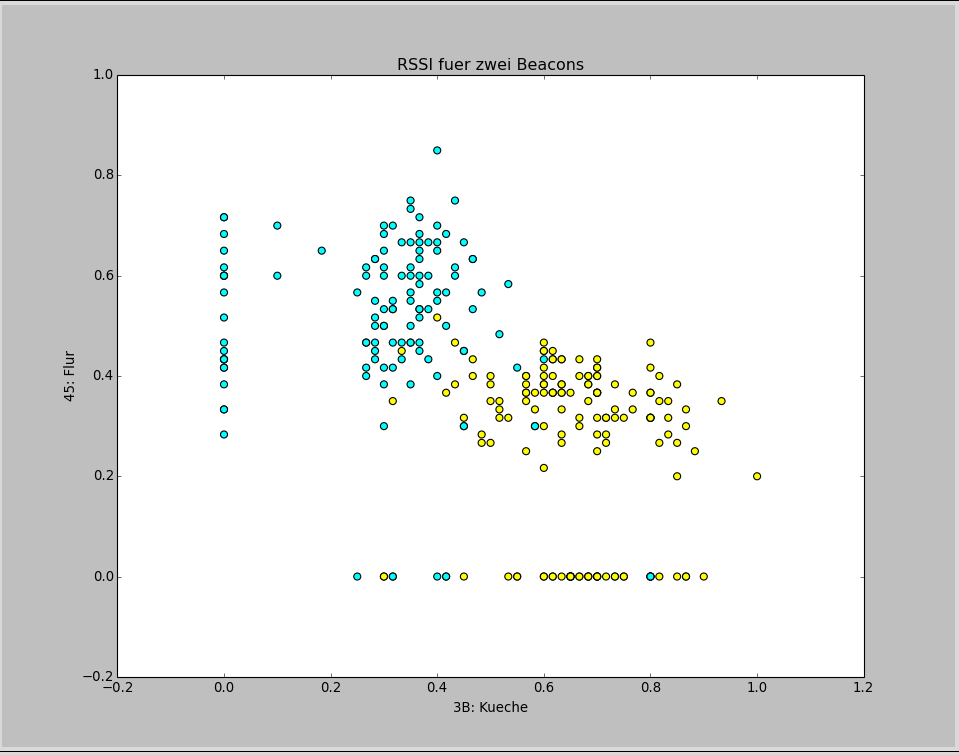
\includegraphics[width=1.0\linewidth]{Bilder/Messungen/KuecheFlur_1}
	\caption{Messung von Küche und Flur mit zwei Beacons}
	\label{fig:KuecheFlur_1}
\end{figure}

\subsection{Lösungsansatz}

Da die Machbarkeitsanalyse mit einem positiven Ergebnis abgeschlossen wurde,
entwickeln wir in diesem Abschnitt einen konkreten Lösungsansatz für die
Raumerkennung auf Basis von Messungen. Dazu erstellen wir ein Modell, dass aus
einer Reihe von Messungen den aktuellen Raum möglichst genau bestimmt.

Das Modell hat zwei Aufgaben:
\begin{enumerate}
	\item Um eine Messung einem Raum zuzuordnen, soll aus dem Messvektor der
		wahrscheinlichste Raum berechnet.
	\item Eine Messung allein reicht nicht aus, um eine korrekte Aussage über
		den aktuellen Raum zu machen. Deshalb sollen mehrere Messungen zu
		einer sicheren Vorhersage zusammengefasst werden
\end{enumerate}

\subsubsection{Bestimmung des wahrscheinlichsten Raums aus einer Messung}
\label{sec:lok-wahrscheinlich}

In Abschnitt \ref{sec:lok-grafische-aufbereitung} haben wir gesehen, dass die
Messungen für unterschiedliche Räume zum großen Teil linear separierbar sind.
Allerdings gilt das nicht für die komplette Menge von Messungen.
Ein naiver Ansatz wie der Perzeptron-Algorithmus würde also nicht zum Erfolg
führen, da der Algorithmus nur konvergiert, wenn die Daten komplett linear
separierbar sind
\footnote{\url{https://www.pearsonhighered.com/assets/hip/us/hip_us_pearsonhighered/samplechapter/0131471392.pdf}}.

Daher wählen wir die etwas mächtigere Softmax-Regression, welche wir an unserer
konkreten Aufgabenstellung vorstellen wollen.
Zunächst definieren wir folgende Symbole:
\begin{itemize}
	\item Anzahl von gemessenen Beacons: $n \in \mathbb{N}$
	\item Anzahl von vermessenen Räumen: $m \in \mathbb{N}$
	\item Messung als Vektor von Einzelmessungen: $ \vec{x} \in [0, 1]^n \subset \mathbb{R}^n $
	\item Einzelmessung für Beacon $i \in [0, n - 1] \subset \mathbb{N}$: $x_i \in [0, 1] \subset \mathbb{R}$
	\item Wahrscheinlichkeitsvektor für alle Räume: $ \vec{y} \in [0, 1]^m \subset \mathbb{R}^m$
	\item Wahrscheinlichkeit für den Raum $j \in [0, m - 1] \subset \mathbb{N}$:
		$ y_j \in [0, 1] \subset \mathbb{R} $ 
\end{itemize}

Der Messvektor $\vec{x}$ enthält die normalisierten Signalstärken für die wahrgenommenen
Bluetooth-Beacon. Er stellt die Eingabe für die Vorhersage dar. 
Der Raumvektor $\vec{y}$ besteht aus den Wahrscheinlichkeiten für die einzelnen Räume und
ist die Ausgabe der Vorhersage. Wichtig ist hier die Eigenschaft, dass sich die Wahrscheinlichkeiten
zu eins addieren:
$$ \sum_{j=0}^{m-1} y_j = 1 $$

Um aus dem Eingabevektor die gewünschte Ausgabe zu erzeugen, sind zwei Schritte notwendig.
Zuerst werden die Komponenten des Eingabevektors gewichtet summiert und mit einem Bias
versehen:

$$ z_j = \sum_{i=0}^{n-1} W_{j,i} \cdot x_i + b_j $$

Die Gleichung kann auch in Matrixform geschrieben werden:

$$ \vec{z} = W \vec{x} + \vec{b} $$

Die neu eingeführten Symbole haben folgende Bedeutung:
\begin{itemize}
	\item $W \in \mathbb{R}^{m \times n}$: Gewichtsmatrix mit $m$ Zeilen und $n$ Spalten
	\item $\vec{b} \in \mathbb{R}^m$: Bias-Vektor mit $m$ Komponenten
	\item $\vec{z} \in \mathbb{R}^m$: Nicht normalisierter Ausgabevektor mit $m$ Komponenten
\end{itemize}

Der nicht normalisierte Vektor $\vec{z}$ kann jetzt über die Softmax-Funktion normalisiert
werden\footnote{\url{http://www.gatsby.ucl.ac.uk/~chuwei/paper/smc.pdf}}:

$$ \vec{y} = \text{softmax}(\vec{z}) $$
$$ y_j = \frac{\exp(z_j)}{\sum_{k=0}^{m-1} \exp(z_k) } $$

Die Gewichtsmatrix $W$ und der Bias-Vektor $\vec{b}$ stellen Parameter der Regression dar,
die durch eine Vermessung der Räume ermittelt werden müssen. Dabei sind die Parameter so
zu wählen, dass möglichst wenig Messungen falsch eingeordnet werden. Dazu definieren wir
eine Verlustfunktion, die ein Maß für die Abweichung von der korrekten Zuordnung darstellt.
Ein Machine-Learning-Algorithmus kann diese Verlustfunktion minimieren, um
gute Parameterwerte zu bestimmen.

Wir haben als Verlustfunktion die Kreuzenthropie gewählt. Dabei werden die vom Modell vorhergesagten
Wahrscheinlichkeiten mit den korrekten Räumen aus der Vermessung kombiniert.
Sei $\vec{y'} \in \mathbb{R}^m$ der erwartete Ausgabevektor für den Raum $r$, dann gilt:
\[
y_j' = 
\begin{cases}
	1 & \text{wenn } j = r  \\ 
	0 & \text{sonst}
\end{cases}
\]
Die Verlustfunktion kann dann wie folgt definiert werden:
$$ \text{Loss}(\vec{y}, \vec{y'}) = - \sum_{j=0}^{m-1} y_j' \cdot \log(y_j) $$

Zu beachten ist, dass die so bestimmten Werte zwar alle mathematischen
Eigenschaften für Wahrscheinlichkeiten erfüllen. Da die konkreten Werte von der
Größe der Parameter $W$ und $\vec{b}$ abhängen, können wir den Ausgabevektor
allerdings nur zur Bestimmung des Raums mit der größten Wahrscheinlichkeit nutzen.

\subsubsection{Zusammenfassung von Messungen}
\label{sec:lok-zusammenfassung-messungen}

Im vorherigen Abschnitt haben wir den wahrscheinlichsten Raum für eine Messung bestimmt.
Da eine Messung keine absolut korrekte Raumerkennung leisten kann, kombinieren wir
die Ergebnisse von mehreren aufeinanderfolgenden Messungen.

Dabei betrachten wir die letzten $N$ Messungen und wählen den Raum, der in diesen
$N$ Messungen am meisten als wahrscheinlichster Raum bestimmt wurde.
Dies hat den Vorteil, dass einzelne Fehlmessungen nicht zu einem spontanem Raumwechsel
führen. Allerdings führt dieses Vorgehen auch eine gewisse Latenz ein, bis ein Wechsel
erkannt werden kann. Deshalb sollte $N$ weder zu klein, noch zu groß gewählt werden.
Ein weiterer Vorteil ist, dass durch diesen Ansatz ein Hysterese-Effekt entsteht.
Befindet sich der Anwender gerade im Übergang zwischen zwei Räumen, wird nicht ständig
ein Raumwechsel gemeldet, sondern erst nach einer kurzen Verzögerung.
  
\subsection{Implementierung}

Bei der Implementierung unseres Lösungsansatzes sind folgende Rahmenbedingungen zu beachten:
\begin{enumerate}
	\item Der Machine-Learning-Algorithmus zur Bestimmung der Parameter des Modells aus
		den Vermessungsdaten ist rechenintensiv und soll deshalb in einen Web-Service
		ausgelagert werden.
	\item Die Vermessung von Räumen und die Erstellung eines Modells soll nur einmalig
		erfolgen, da die Smartwatch-App ansonsten auch offline funktionsfähig sein soll.
	\item Die Anwendung des gelernten Modells auf Messungen bei der Raumerkennung muss
		performant sein, da diese Berechnung lokal auf der Smartwatch erfolgt.
\end{enumerate}

\subsubsection{Web-Service}

Um den Machine-Learning-Algorithmus zu implementieren, haben wir uns für
TensorFlow\footnote{\url{https://www.tensorflow.org/}} entschieden.
Da diese API primär für Python entwickelt wurde, verwenden wir Python auch
für unseren Web-Service.

Der Web-Service wird als einfaches CGI-Skript in einem Apache-Server ausgeführt.
Als Eingabe werden UTF-8-kodierte Vermessungsdaten im CSV-Format erwartet.
Nachdem die Daten normalisiert und aufbereitet wurden, erstellen wir das
zuvor entwickelte Berechnungsmodell (siehe \ref{sec:lok-wahrscheinlich}) in
TensorFlow. Anschließend wird der Machine-Learning-Algorithmus auf die
Vermessungsdaten angewendet.
Das berechnete Modell wird im JSON-Format an den Client gesendet.

Das Modell enthält folgende Daten:
\begin{itemize}
	\item Gelernte Parameter: $W$, $\vec{b}$
	\item Normalisierungsinformationen: $max_{RSSI}, min_{RSSI}$
	\item Zuordnung der Beacon-Adressen und Raum-IDs zu Indizes in den Vektoren
\end{itemize}
Die Normalisierungsinformationen sind wichtig, um bei einer Messung die RSSI-Werte in
das erforderliche Intervall $[0, 1] \subset \mathbb{R}$ zu überführen.
Um beliebige Beacon-Adressen auf die korrekten Positionen im Eingabevektor $\vec{x}$
und die Komponenten im Ausgabevektor $\vec{y}$ wieder auf die betroffenen Raum-IDs
zu mappen, sind zusätzliche Zuordnungsinformationen im Modell enthalten.

\subsubsection{Offline-Fähigkeit}

Die Berechnung des Modells erfolgt im besten Fall einmalig nach Vermessen aller Räume.
Das so erstellte Modell soll auch ohne Verbindung zum Smartphone oder Internet von
der Smartwatch angewendet werden. Deshalb speichern wir das Modell als serialisiertes
Java-Objekt in den Einstellungen der Smartwatch-App über der Preferences-API
\footnote{\url{https://developer.android.com/reference/android/preference/Preference.html}}.
Da die Daten nicht relational sind, haben wir uns gegen das Ablegen in der Datenbank
entschieden.

\subsubsection{Anwendung des Modells}

Da das Modell performant auf die eingehenden Messdaten angewendet werden soll,
implementieren wir die Vektoren und Matrizen als ein- bzw. zweidimensionale
Floating-Point-Arrays. Alle Berechnungen sind in der Klasse PredictionModel
implementiert.

Die Zusammenfassung von mehreren Messungen auf eine Raumvorhersage
(siehe \ref{sec:lok-zusammenfassung-messungen}) erfolgt durch die Implementierung
einer beschränkten Queue, wobei wir als maximale Länge $N = 10$ gewählt haben.

